\documentclass[multi=tikzpicture,border=8pt]{standalone}
\usepackage[UTF8]{ctex}
\usepackage{amsmath,amssymb,tikz}
\usetikzlibrary{arrows.meta,calc,decorations.pathmorphing}
\definecolor{blue}{HTML}{17365D}
\definecolor{red}{HTML}{AC3931}
\tikzset{every node/.style={font=\small},arrow/.style={-{Stealth[length=2.8mm]},thick},dim/.style={|<->|,thin},box/.style={draw,rounded corners,align=center,minimum width=2.5cm,minimum height=.9cm}}
\begin{document}
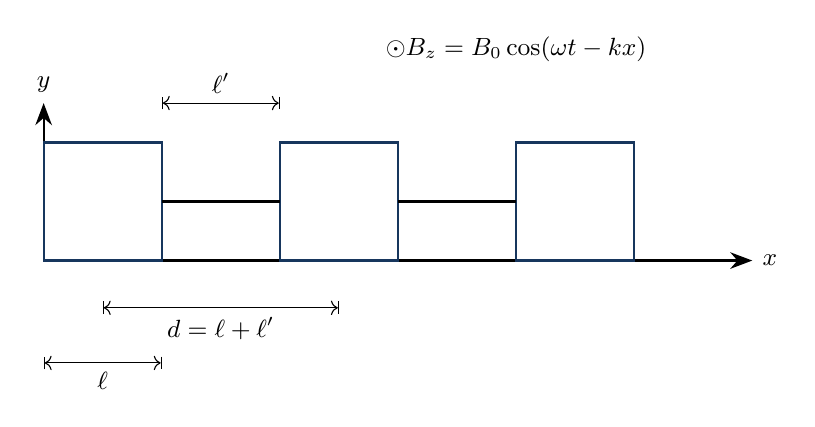
\begin{tikzpicture}

\draw[arrow](0,0)--(9,0)node[right]{$x$};\draw[arrow](0,0)--(0,2)node[above]{$y$};\draw[thick,blue](0,0)rectangle(1.5,1.5);\draw[thick,blue](3,0)rectangle(4.5,1.5);\draw[thick,blue](6,0)rectangle(7.5,1.5);\draw[very thick](1.5,.75)--(3,.75);\draw[very thick](4.5,.75)--(6,.75);\draw[dim](1.5,2)--(3,2)node[above,midway]{$\ell'$};\draw[dim](.75,-.6)--(3.75,-.6)node[below,midway]{$d=\ell+\ell'$};\draw[dim](0,-1.3)--(1.5,-1.3)node[below,midway]{$\ell$};\node[above]at(6,2.4){$\odot B_z=B_0\cos(\omega t-kx)$};

\end{tikzpicture}
\begin{tikzpicture}
\draw[arrow](0,0)--(7.4,0)node[right]{$kX$};\draw[arrow](0,0)--(0,3.4)node[above]{$B_z/B_0$};
\fill[blue!10](1,-2)rectangle(4,2);\draw[blue,very thick,domain=0:7,samples=100]plot(\x,{2*cos((\x-2.2) r)});\draw[dashed](1,-2)--(1,2.5);\draw[dashed](4,-2)--(4,2.5);\node[above]at(1,2.5){左边};\node[above]at(4,2.5){右边};\draw[dim](1,-2.5)--(4,-2.5)node[midway,below]{$k\ell$};\node[left]at(0,2){1};\node[left]at(0,-2){$-1$};

\end{tikzpicture}
\begin{tikzpicture}

\node[box](a)at(0,1.3){变磁通电动势\\$\mathcal E_t\propto\omega$};\node[box](b)at(0,-1.3){运动电动势\\$\mathcal E_v\propto-kv$};\node[box,fill=blue!8](c)at(5,0){总电动势\\$\mathcal E\propto\omega-kv$};\draw[arrow](a)--(c);\draw[arrow](b)--(c);\node[below]at(2.5,-2.7){$v=\omega/k$时，两种电动势抵消};

\end{tikzpicture}
\begin{tikzpicture}
\draw[arrow](0,0)--(7.4,0)node[right]{$\xi$};\draw[arrow](0,0)--(0,4.4)node[above]{$F_x/(C\Omega)$};
\draw[blue,very thick,domain=0:6.28318,samples=120]plot(\x,{4*sin(\x r)^2});\draw[red,dashed](0,2)--(6.5,2)node[right]{平均$1/2$};\node[left]at(0,4){1};\node[left]at(0,0){0};\foreach \x/\t in {0/0,3.14159/\pi,6.28318/{2\pi}}{\node[below]at(\x,0){$\t$};}\node[above]at(3.1,4.4){每个周期都出现零磁力};

\end{tikzpicture}
\begin{tikzpicture}

\draw[gray](0,0)circle(1.8);\foreach \a/\t in {0/{1},120/{e^{-2ikd}},240/{e^{-4ikd}}}{\draw[arrow,blue](0,0)--({1.8*cos(\a)},{1.8*sin(\a)})node[above]{$\t$};}\node[below]at(0,-2.5){三个二倍频相量之和为零};\draw[arrow](4,-.5)--(9,-.5)node[right]{$\xi$};\draw[arrow](4,-.5)--(4,2.5)node[above]{$F_{\rm tot}/(C\Omega)$};\draw[very thick,red](4,1.5)--(9,1.5)node[right]{$3/2$};\node[align=center]at(6.5,-1.7){总力恒定\\$kd=\pi/3$或$2\pi/3\pmod\pi$};

\end{tikzpicture}
\end{document}
